%--
%-- Modelo de Objetivos
%--
\clearpage
\subsection{Modelo de Objetivos}

\subsubsection{Listado de objetivos}

\paragraph{1 - Objetivo primario}

El objetivo primario del sistema es revertir la disminución de ventas (1) que se
viene produciendo en la cadena de supermercados hace meses. Para ello, se nos
brinda la información de que las dos causas de las disminuciones son las largas
colas en el supermercado y el agotamiento del stock (1.3), de donde se
desprenden los objetivos (1.1) y (1.2).

\paragraph{1.1 - Reducción de colas}

Dentro del contexto de la reducción de colas, se tomó la presunción de que cada
venta online estaría disminuyendo las colas en la sucursal (1.1.2), dado que de
este modo ese cliente, que normalmente estaría haciendo cola en el supermercado,
puede encargar los productos desde la comodidad de su casa. De este modo, se
toma el objetivo de permitir que el usuario compre de forma online (1.1.1).

\paragraph{1.1.1 - Permitir al usuario la compra online}

Consideramos que para permitir que el cliente compre un pedido de forma online,
deben ocurrir dos cosas, lograr que el cliente encargue el pedido (1.1.1.1)
\footnote{lo cual incluye todo el proceso desde que el cliente se registra en
el sitio, realizando la selección de productos, acordando una fecha de entrega y
eligiendo una forma de pago}, y lograr que el pedido sea cerrado y finalizado
(1.1.1.2), que comienza con la confirmación del pedido por parte del cliente, y
culmina con la entrega del pedido (o la cancelación/anulación, según el caso).

\clearpage
\paragraph{1.1.1.1 - Lograr[Cliente encarga pedido]}

Para que un cliente encargue un pedido, es necesario que el mismo pueda
identificarse en el sistema (1.1.1.1.1), que el pedido sea armado (1.1.1.1.2),
que se pueda acordar una fecha de entrega (1.1.1.1.3), una forma de pago
(1.1.1.1.4) y que si esta última es online, se le pueda cobrar.

\paragraph{1.1.1.1.1 - Lograr[Cliente identificado]}

Para que el cliente pueda ser identificado por el sistema, es necesario que se
encuentre registrado (1.1.1.1.1.1), y que se autentique (1.1.1.1.1.2)

\paragraph{1.1.1.1.1.1 - Lograr[Cliente registrado]}

La forma en que un cliente se registra es uno de los o-refinamientos
propuestos. Dividimos el registro entre online y presencial. El registro
online implica que el cliente se conecte al sitio, cargando sus datos
personales, y sus datos de pago, los cuales son verificados por el sistema al
momento de la registración. El registro presencial, en cambio, requiere que el
cliente se dirija a la sucursal con la documentación necesaria para verificar
identidad, domicilio y datos de pago, los cuales son archivados y verificados
por un empleado de la sucursal, y posteriormente cargados al sistema. Más
pormenores sobre este refinamiento, junto con la justificación del puntaje
asignado a los objetivos blandos, están explicados posteriormente.

\paragraph{1.1.1.1.1.2 - Lograr[Cliente se autentica de forma segura]}

La autenticación requiere que el cliente ingrese sus credenciales
(1.1.1.1.1.2.1). Por otro lado, también es necesario proveer una interfaz que
cuente con los mecanismos de seguridad adecuados (1.1.1.1.1.2.2), por ejemplo
conexión HTTPS.

\paragraph{1.1.1.1.2 - Lograr[Armado de pedido]}

Para que el pedido sea armado, consideramos que es necesario que el cliente
pueda ver el stock disponible para cada producto (1.1.1.1.2.1), y que logre
seleccionar la mercadería adecuada (1.1.1.1.2.3). Para ello, planteamos el
objetivo de mostrar recomendaciones personalizadas para cada cliente
(1.1.1.1.2.2), que varían según los distintos datos relacionados a su usuario,
como pueden ser, perfil de comprador, generado a través del historial de
compras, compras de otros clientes, relacionados según escala socioeconómica,
edad, domicilio, etc.

\paragraph{1.1.1.1.3 - Lograr[Acordar fecha de entrega]}

En el transcurso del armado del pedido, es necesario que el cliente acuerde una
fecha de entrega. Para ello, es necesario que el sistema le ofrezca un rango de
fechas disponibles (1.1.1.1.3.2), las cuales serán calculadas e informadas por
logística (1.1.1.1.3.1), y obtenidas en tiempo real, de algun modo, por ejemplo
a través de algún tipo de interfaz entre nuestro sistema y el sistema de
logística. En caso de no haberla, será necesario contar con una forma de
calcularla. Luego de mostrarles las fechas, el cliente eligirá (1.1.1.1.3.3) la
que más le convenga.

\paragraph{1.1.1.1.4 - Lograr[Acordar forma de pago]}

Además de que el cliente seleccione la fecha de entrega, es necesario que
acuerde con el sistema una forma de pago. Para ello, el sistema deberá informar
al cliente cuales son las formas de pago que tiene disponibles (1.1.1.1.4.2), y
el cliente deberá elegir entonces la que le resulte de su conveniencia
(1.1.1.1.4.3). Hay un o-refinamiento aquí, sobre el objetivo de evaluar si se
deberá permitir la contraentrega.

\paragraph{1.1.1.1.4.1 - Lograr[Evaluar si permitir contraentrega]}

Para evaluar si el cliente puede realizar un pedido por contrareembolso,
proponemos dos opciones.

La primera de ellas es un límite de entregas fallidas (1.1.1.1.4.1.1), contenido
dentro de la programación del sistema, e instanciado en 1 en nuestros ejemplos,
es decir, se limita la posibilidad de que el cliente no esté presente en la
última entrega. Llegado tal caso, se le bloqueará la modalidad contraentrega
(1.1.1.1.4.1.1.1) y se ofrecerá el pago de una multa (1.1.1.1.4.1.1.2) para
poder desbloquearla (1.1.1.1.4.1.1.3). El valor de la multa, además, no es fijo,
sino que dependerá directamente del costo del envío al domicilio de ese cliente
en particular (1.1.1.1.4.1.1.2.1.1), y el costo de la mercadería que no pudo ser
reingresada a stock (1.1.1.1.4.1.1.2.1.2). Se le ofrecerán dos modalidades de
pago, pagar en efectivo al momento de recibir el envío de un pedido distinto
(1.1.1.1.4.1.1.2.2.1) o pagar online (1.1.1.1.4.1.1.2.2.2).

La segunda opción es un límite de pérdida de redituabilidad (1.1.1.1.4.1.2).
Para ello, el Administrador deberá definir previamente un umbral de pérdida de
redituabilidad (1.1.1.1.4.1.2.1), el cual el sistema deberá segurarse de que sea
respetado en todo momento (1.1.1.1.4.1.2.2). En caso de que el cliente produzca
costos de tal forma que la redituabilidad se encuentre por bajo del umbral, la
contraentrega deberá bloquearse (1.1.1.1.4.1.2.2.3). Para ello, es necesario
contabilizar las ganancias (1.1.1.1.4.1.2.2.1) y costos (1.1.1.1.4.1.2.2.2)
generados por el cliente. La redituabilidad, entonces, es una relación
ganancia/costo, la cual no deberá bajar más allá del umbral definido
previamente.

Ambas opciones están detalladas más adelante, junto con la asignación de
puntajes a los objetivos blandos.

\paragraph{1.1.1.1.5 - Lograr[Si la forma de pago es online, cobrar]}

Si el cliente elige el pago online, además, hay que cobrarle. Para ello, se
cuenta con la participación del cliente, el cual deberá validarse a través del
agente de cobro, para que el importe le sea deducido de su cuenta bancaria.

\clearpage
\paragraph{1.1.1.2 - Lograr[El pedido es finalizado y cerrado]}

Una vez que un pedido está encargado, es necesario que el mismo sea cerrado.
Aquí pueden ocurrir dos cosas, que el usuario cancele el pedido antes de que el
mismo sea preparado (1.1.1.2.2), caso en el que el mismo se anula y se le
devuelve el dinero, o que el usuario confirme el pedido (1.1.1.2.1). En este
último caso, será necesario preparar el pedido (1.1.1.2.1.1) a la vez que el
stock es restado del conteo del sistema (1.1.1.2.1.2), y luego lograr que el
mismo sea entregado a logística (1.1.1.2.1.3). Además de todo esto, será
necesario asegurar que el envío sea realizado (1.1.1.2.1.4).

\paragraph{1.1.1.2.1.4 - Lograr[Realizar el envío]}

Al momento de realizar el envío, pueden ocurrir dos situaciones, o que el
cliente reciba el pedido (1.1.1.2.1.4.1), o que no lo reciba (1.1.1.2.1.4.2).
Por simplicidad, se englobaron todas las situaciones en las que el cliente puede
no recibir el pedido, en una situación ``el cliente no está presente''. Es
decir, también es este el caso cuando un cliente esta presente pero por alguna
razón se niega a recibir el pedido.

\paragraph{1.1.1.2.1.4.2 - Lograr[Realizar el envío]}

En caso de que el cliente no reciba el pedido, será necesario deshacer la
operación, es decir, reintegrar el dinero de ser necesario (1.1.1.2.1.4.2.1),
marcar el pedido como no recibido en el historial del cliente (1.1.1.2.1.4.2.2),
y que logística devuelva el stock al depósito para que sea reingresado
(1.1.1.2.1.4.2.3). Esto significa que Depósito realizará la evaluación de los
productos (ya que algunos pueden haberse roto o perdido su calidad en el
transcurso del envío), y reingresará a stock los que considera que se encuentran
adecuados. Además, se le informará al cliente que su pedido no fue recibido
mediante un email, y se le ofrecerá rehacerlo (1.1.1.2.1.4.2.4).

\clearpage
\paragraph{1.2 - Mantener[Stock disponible]}

Para mantener el stock disponible, se deberá mantener el stock disponible tanto en las sucursales (1.2.1) como en los depósitos (1.2.2)

\paragraph{1.2.1 - Mantener[Stock disponible en sucursales]}

Para mantener el stock disponible en las sucursales es necesario lograr realizar un conteo periódico del stock en las sucursales (1.2.1.1), y encargar una reposición por medio del sistema en cuanto el stock sea bajo (1.2.1.2). Por otro lado, será necesario lograr que el depósito sea informado en cuanto haya un pedido nuevo (1.2.1.3). Respecto a esto, la idea es que el depósito mantenga un sistema interno propio que cuente con acceso a la misma base de datos que el sistema web. Tamibén es necesario armar el pedido, y entregarlo a logística (1.2.1.4), de esto se encargaría el depósito. Finalmente, logística debe entregar la reposición de stock a la sucursal (1.2.1.5).

\paragraph{1.2.2 - Mantener[Stock disponible en depósitos]}

Para poder mantener el stock en el depósito, es necesario contar con un límite mínimo de productos, de forma tal de asegurarse de que cada producto se encuentre siempre por encima de este límite (1.2.2.2). Como cada producto es distinto del otro, y tienen distintos ritmos de ventas, este límite no puede ser igual para todos los productos, ni puede estar contenido dentro del código del programa. Para determinar este límite, entonces, será necesario contar con una forma de modificar los productos y sus límites, según las estadísticas de ventas de cada uno (1.2.2.1).

\paragraph{1.2.2.1 - Lograr[Modificar productos y sus límites según estadísticas]}

Por un lado se ofrece la capacidad típica de agregar nuevos productos, modificar los existentes, o dar de baja otros (ABM, 1.2.2.1.1). Utilizando esta interfaz, el administrador deberá modificar los productos, estipulando el límite inferior de stock para cada uno de ellos (1.2.2.1.3). Para ayudarlo, el sistema le ofrece estadísticas elaboradas sobre el registro de cada transacción de los clientes. Se puede visualizar la información de manera interactiva y se pueden aplicar herramientas avanzadas de \textit{machine learning} sobre los datos (1.2.2.1.2).

\paragraph{1.2.2.2 - Mantener [Stock de cada producto por encima de límite estipulado por empresa]}

El sistema monitorea constantemente el stock de cada producto, y cuando uno de estos desciende por debajo del límite estipulado, se inicia un proceso de reabastecimiento. Como el producto no está en suficiente cantidad en nuestros depósitos, es necesario recurrir al Departamento de Stock (1.2.2.2.1) que se encarga de conseguir el producto a través de los distintos proveedores, los cuales serán encomendados para su entrega a la logística (1.2.2.2.2). Luego se inicia un proceso logístico que culmina con el producto en el depósito (1.2.2.2.3), y el nuevo stock ingresado al sistema (1.2.2.2.4).

%--
%-- Modelo de objetivos - Diagramas
%--
\subsubsection{Diagramas de Objetivos}
\vspace{-10em}
\begin{figure}[ht]

  \begin{center}

  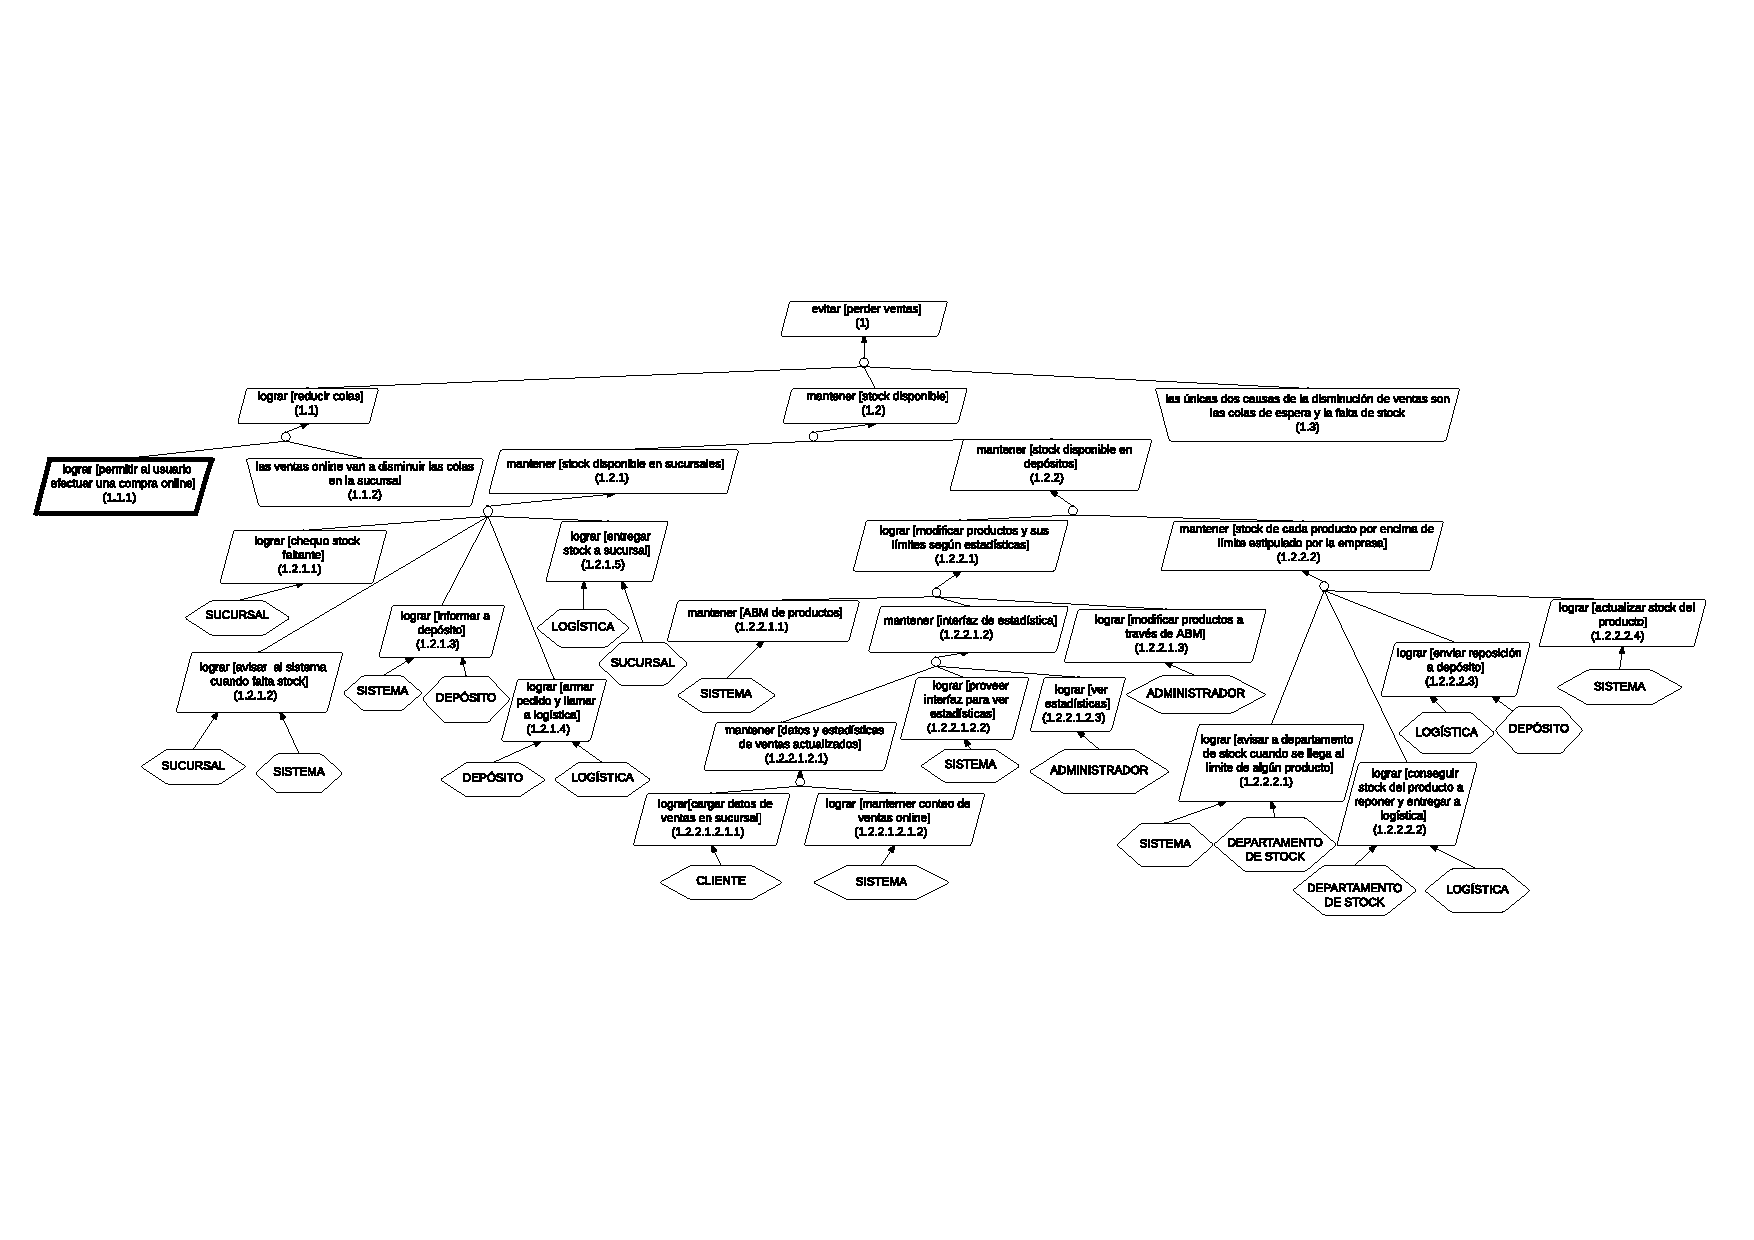
\includegraphics[angle=90,height=\textheight]{images/objetivos-raiz.pdf}
  \caption{Objetivo: Evitar perder ventas}
  \end{center}
\end{figure}

\begin{figure}[ht]
  \begin{center}
  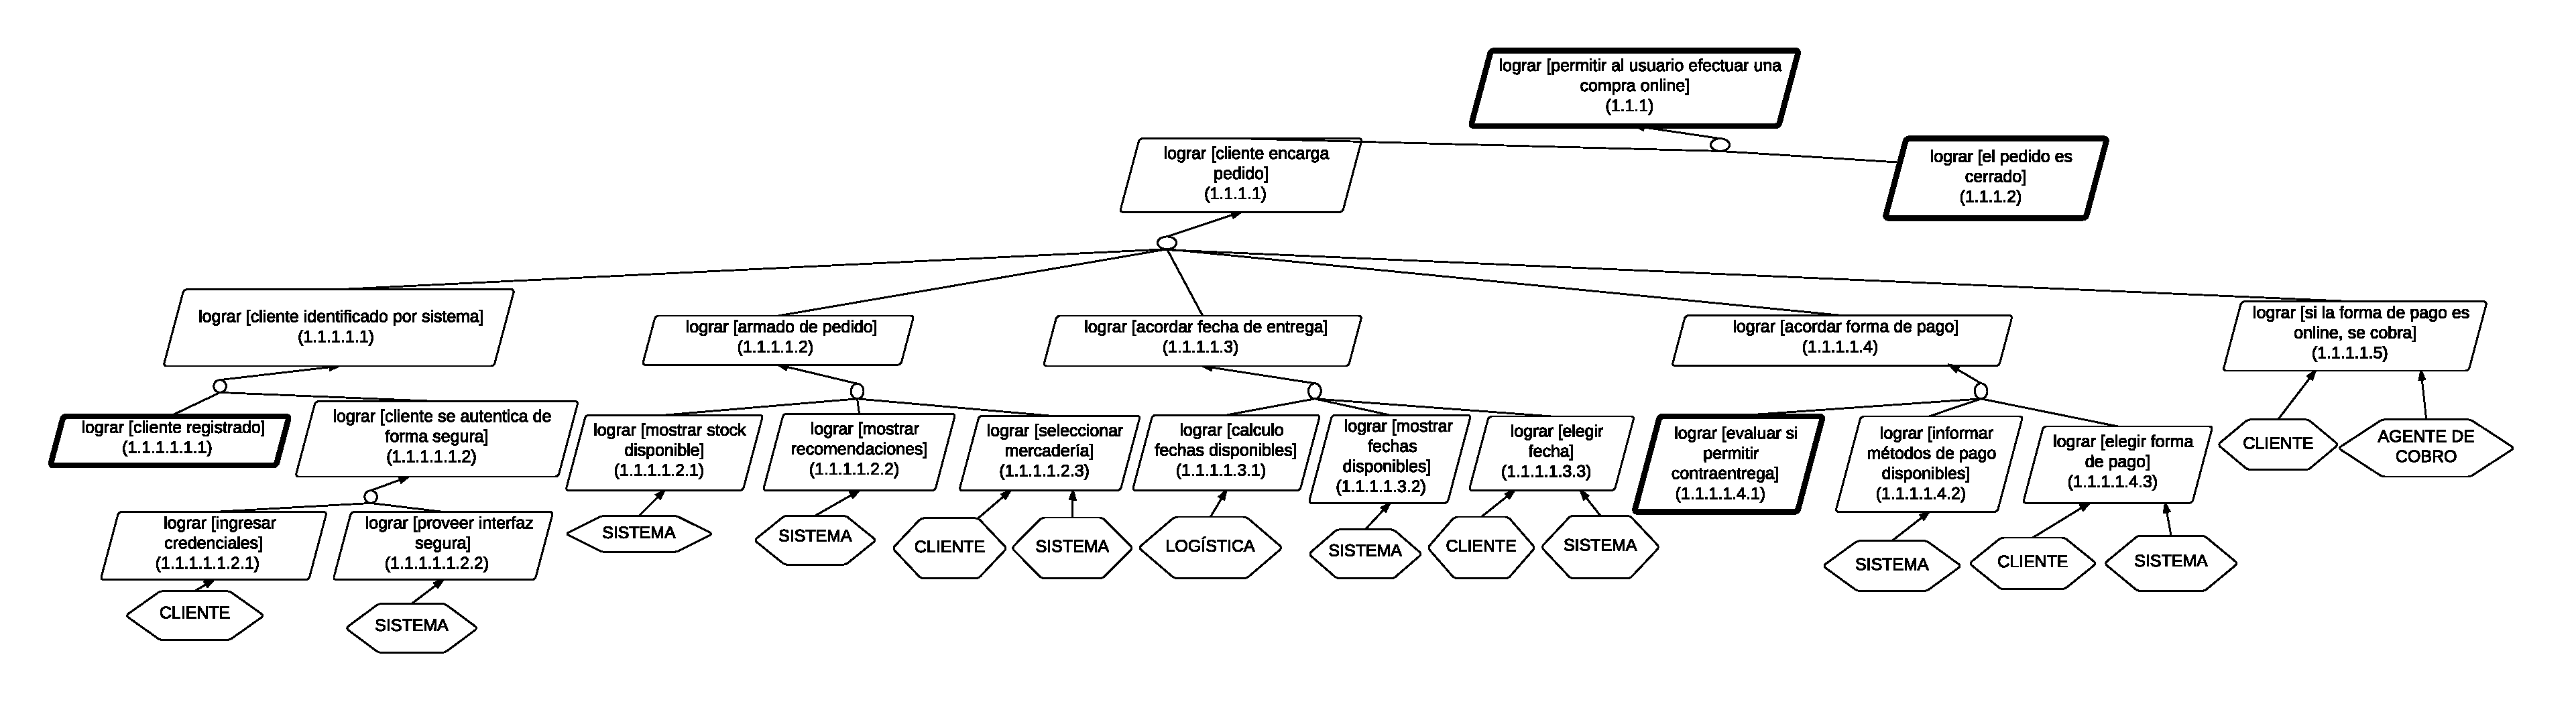
\includegraphics[angle=90,height=\textheight]{images/objetivos-operacion-online.pdf}
  \caption{Objetivo: Lograr permitir al usuario efectuar una compra online}
  \end{center}
\end{figure}

\begin{figure}[ht]
  \begin{center}
  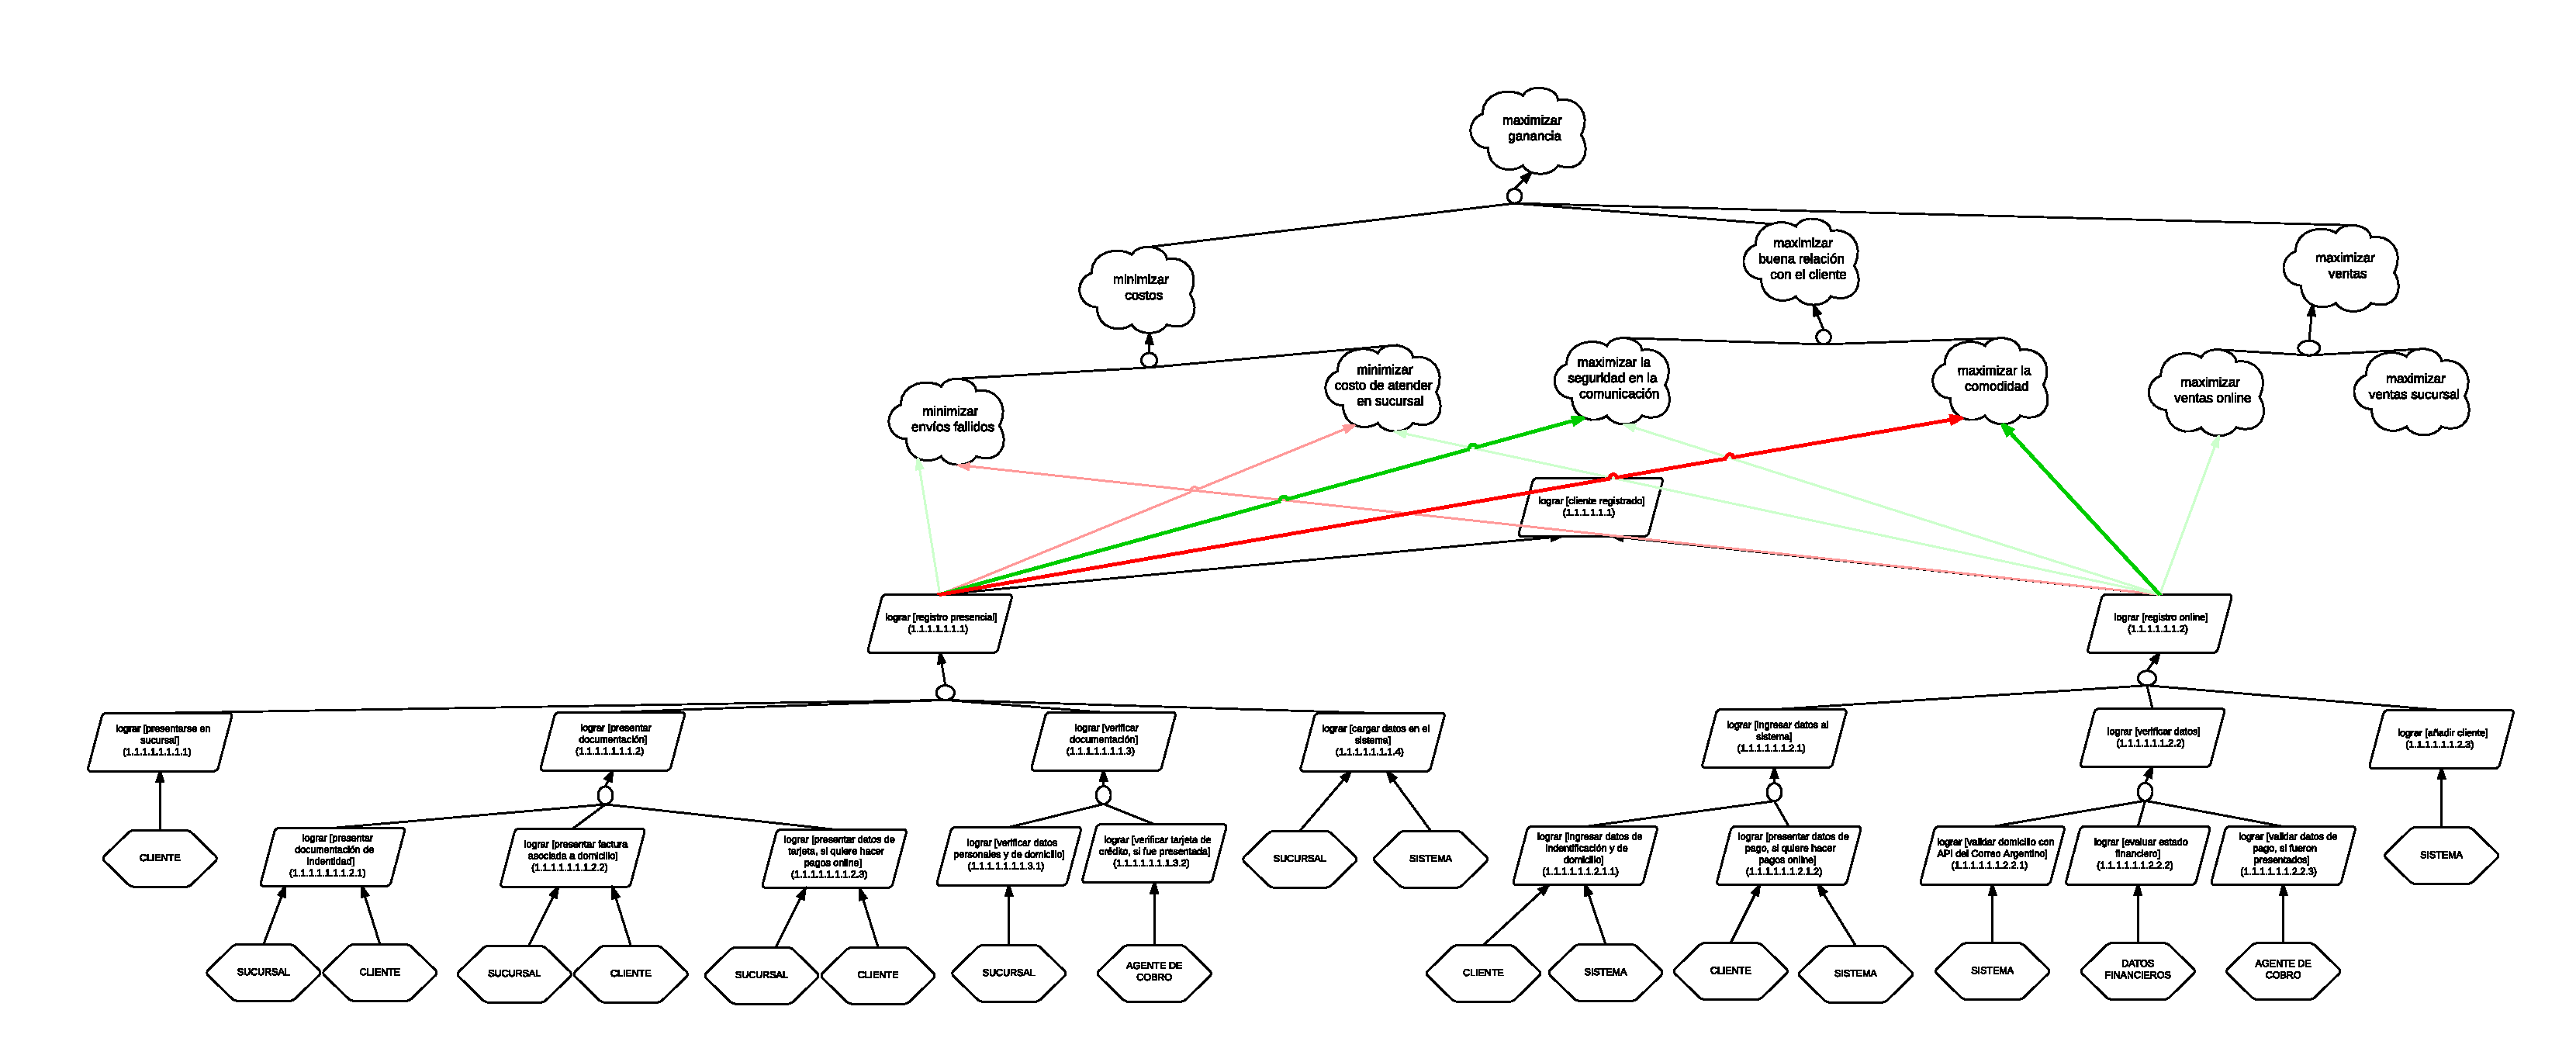
\includegraphics[angle=90,height=\textheight]{images/objetivos-cliente-registrado.pdf}
  \caption{Objetivo: Lograr cliente registrado}
  \end{center}
\end{figure}

\begin{figure}[ht]
  \begin{center}
  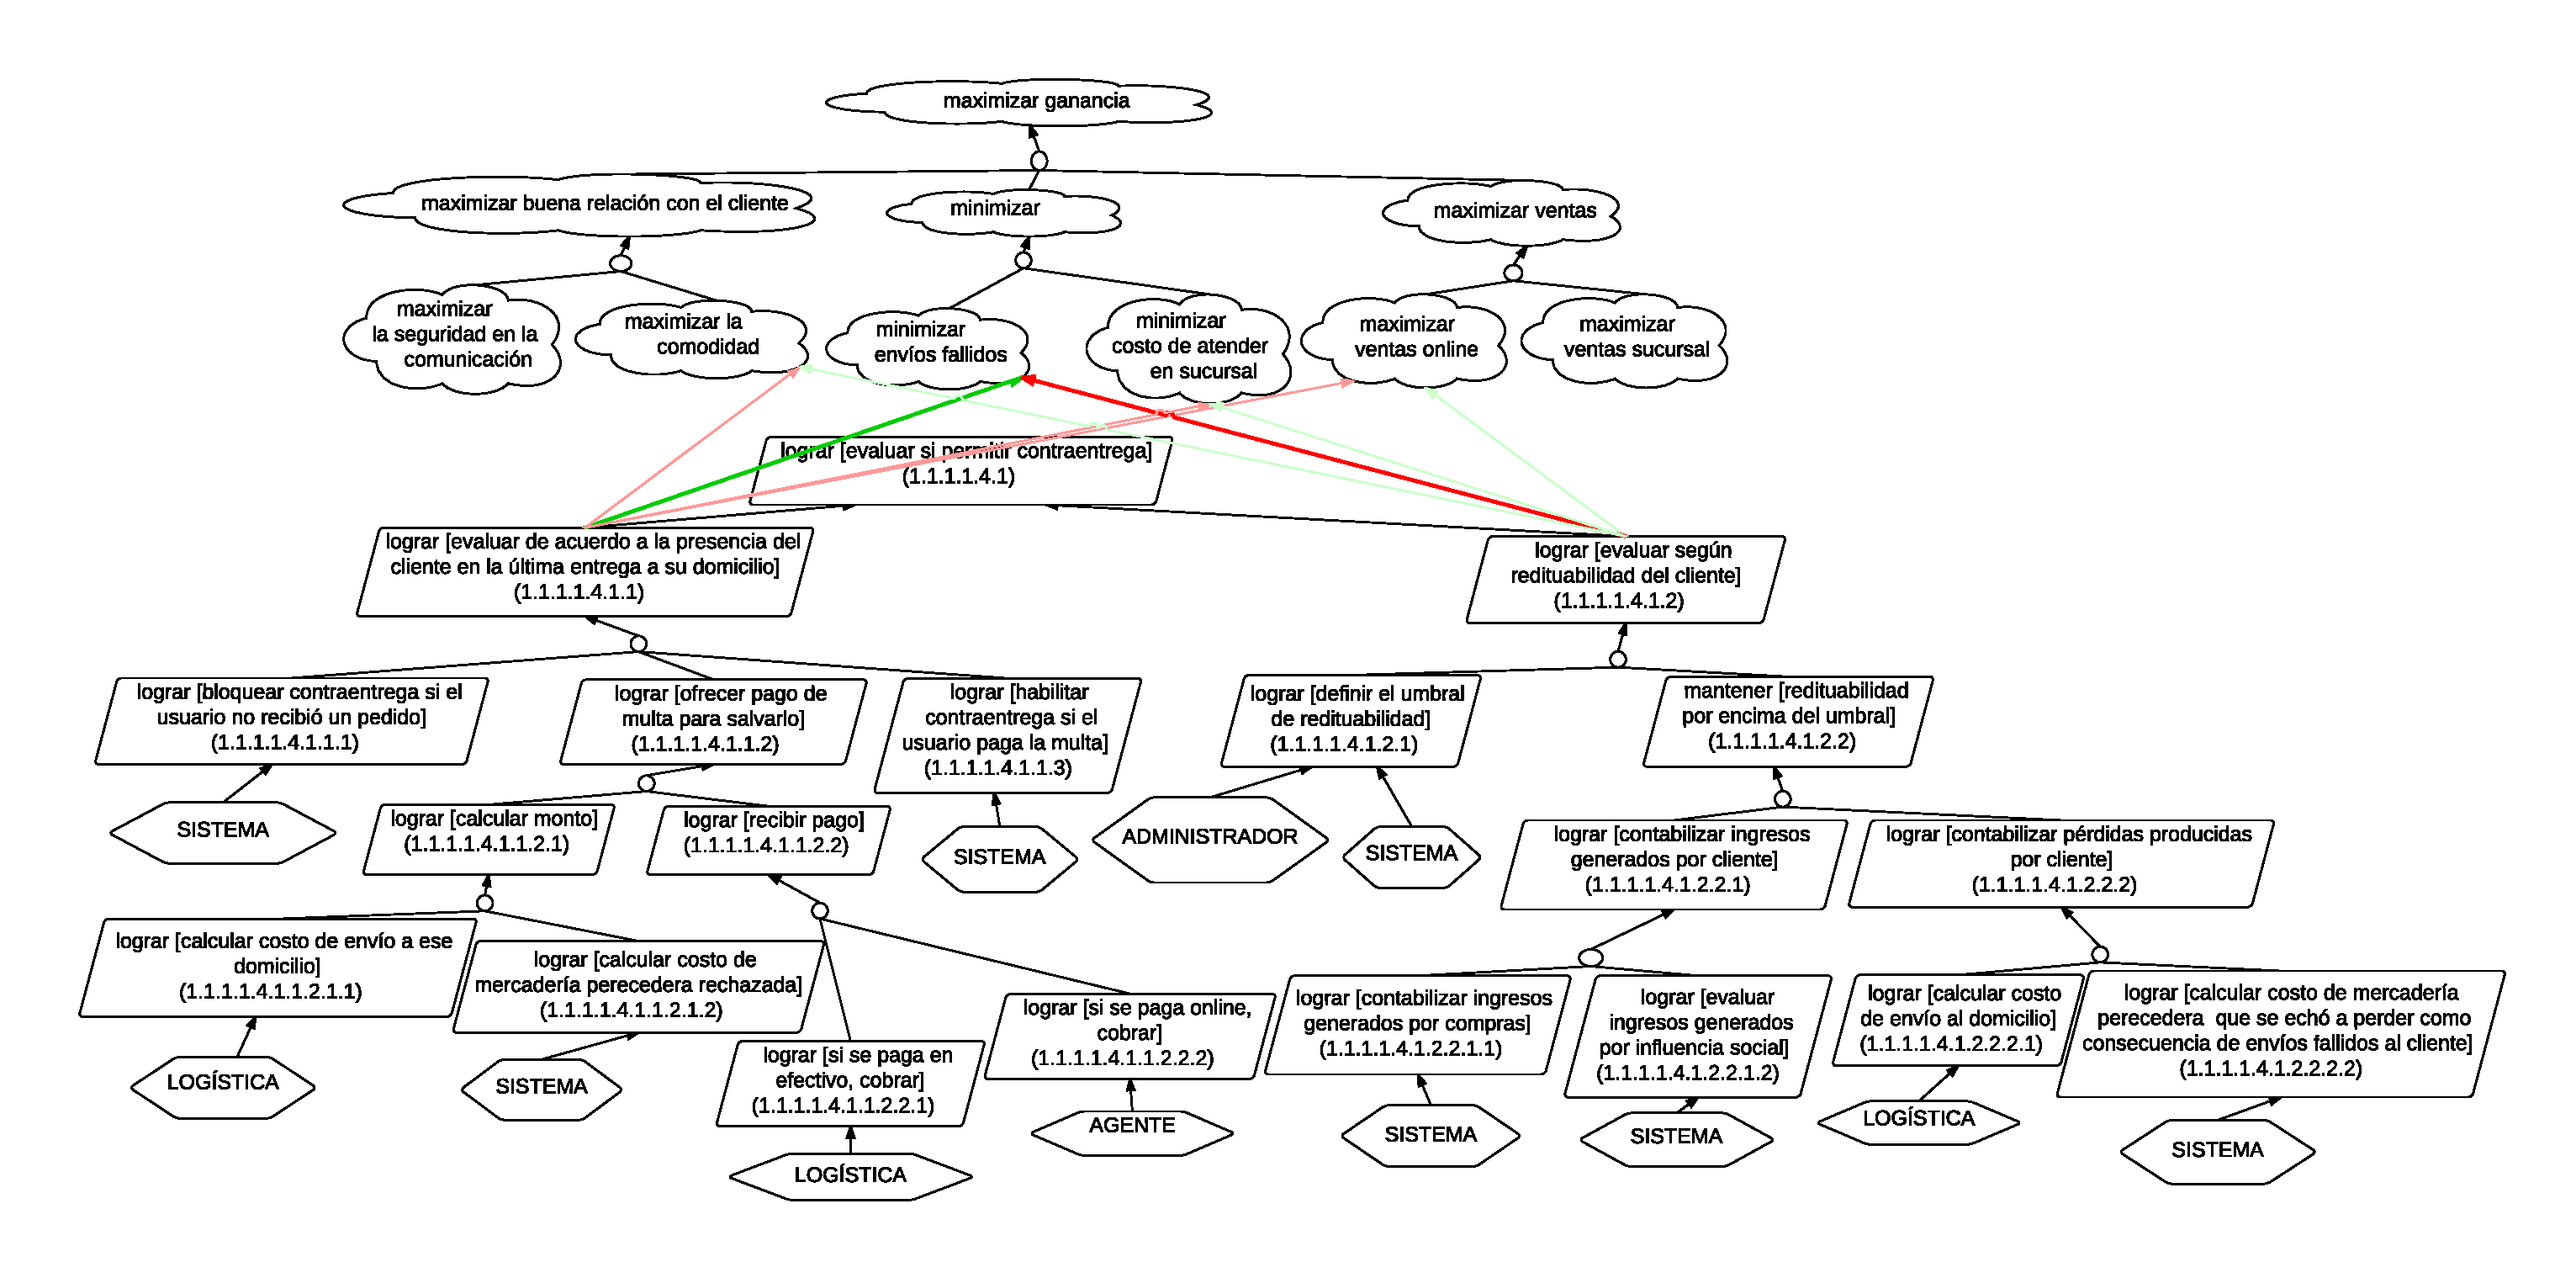
\includegraphics[angle=90,height=\textheight]{images/objetivos-permitir-contraentrega.pdf}
  \caption{Objetivo: Lograr evaluar si permitir contraentrega}
  \end{center}
\end{figure}

\begin{figure}[ht]
  \begin{center}
  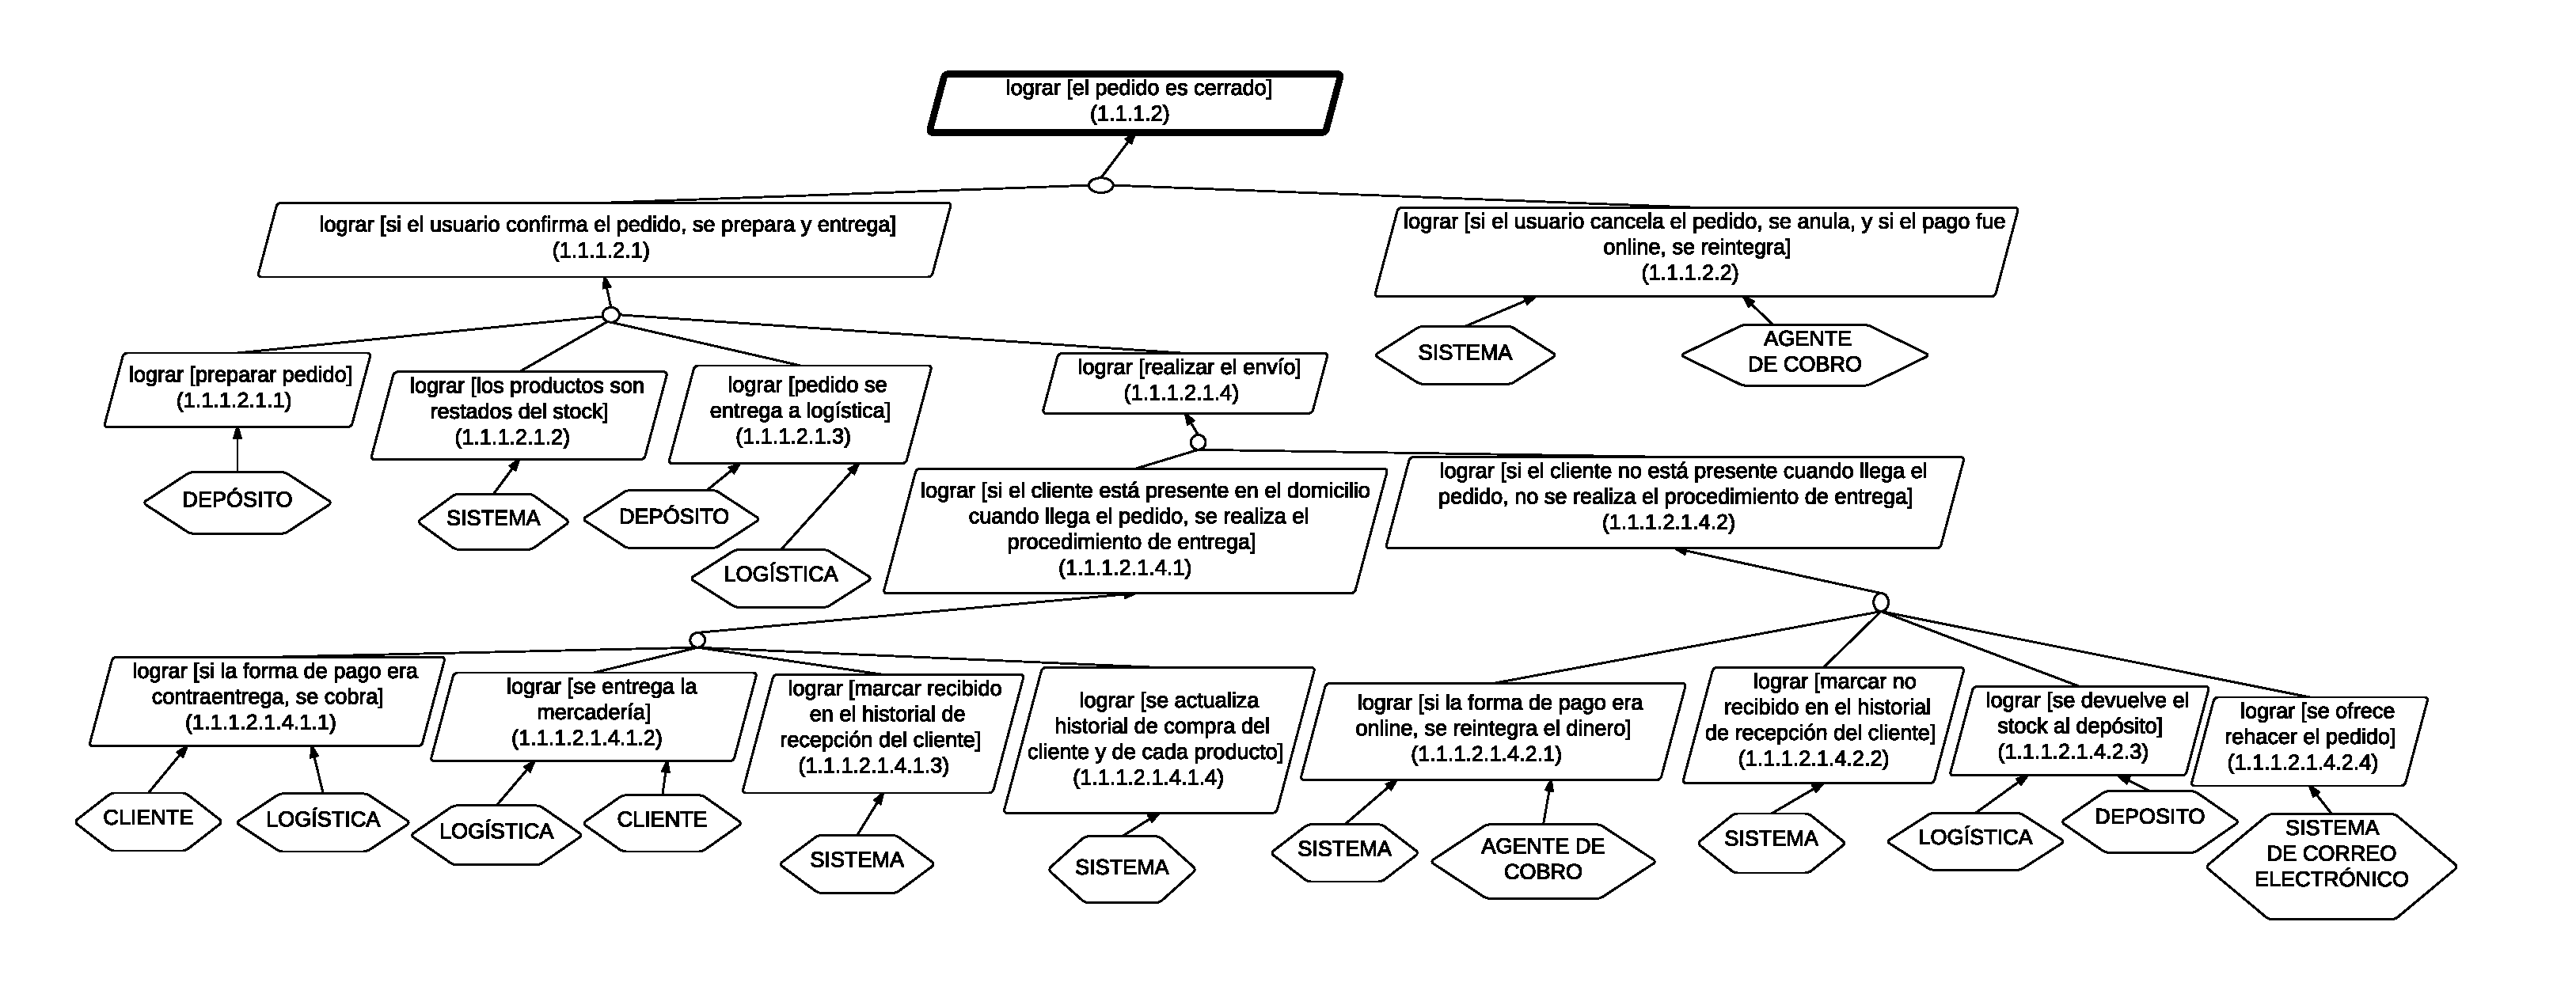
\includegraphics[angle=90,height=\textheight]{images/objetivos-cerrar-pedido.pdf}
  \caption{Objetivo: Lograr el pedido es cerrado}
  \end{center}
\end{figure}
